\section{Propagation Equation and Population Rate Equations}
\subsection{Slow Varying Approximation, Extended Nonlinear Schrödinger Equation}

We start by writing the Maxwell equations in a dielectric medium, taking into account the free charge sources (plasma and ions) generated by the intense laser pulse.
\begin{align}
\nabla \times \vec{B} &= \mu_0 \left( \vec{j} + \frac{\partial \vec{D}}{\partial t} \right) \\
\nabla \times \vec{E} &= -\frac{\partial \vec{B}}{\partial t} \\
\nabla \cdot \vec{B} &= 0 \\
\nabla \cdot \vec{D} &= 0 \quad
\end{align}

We can express the displacement vector by separating its linear and non-linear components. The linear part accounts for the material's dispersion via the frequency-dependent relative permittivity $\varepsilon(\omega)$:
\begin{align}
\vec{D}(\omega, r) &= \varepsilon_0 \vec{E}(\omega, r) + \vec{P}(\omega, r) \nonumber \\
&= \varepsilon_0 \vec{E} + \vec{P}_L + \vec{P}_{NL} \nonumber \\
&= \varepsilon_0 \left(1 + \chi^{(1)}\right) \vec{E} + \vec{P}_{NL} \nonumber \\
&= \varepsilon_0 \varepsilon(\omega) \vec{E}(\omega) + \vec{P}_{NL}(\omega) \nonumber \\
&= \vec{D}_{lin} + \vec{P}_{NL}
\end{align}

Let's derive the propagation equation by applying the curl operator ($\nabla \times$) to Faraday's law of induction. Using the vector identity $\nabla \times (\nabla \times \vec{E}) = \nabla(\nabla \cdot \vec{E}) - \nabla^2 \vec{E}$, and assuming no macroscopic free charges alter the divergence of the electric field ($\nabla \cdot \vec{E} = 0$), we obtain:
\begin{equation}
\nabla \times (\nabla \times \vec{E}) = \underbrace{\cancel{\nabla(\nabla \cdot \vec{E})}}_{\text{No sources}} - \nabla^2 \vec{E} = -\frac{\partial}{\partial t} (\nabla \times \vec{B}) = -\mu_0 \frac{\partial \vec{j}}{\partial t} - \mu_0 \frac{\partial^2 \vec{D}}{\partial t^2}
\end{equation}

This yields the fundamental wave equation:
\begin{equation}
\nabla^2 \vec{E} = \mu_0 \frac{\partial^2}{\partial t^2} \vec{D}_{lin} + \mu_0 \frac{\partial^2}{\partial t^2} \vec{P}_{NL} + \mu_0 \frac{\partial \vec{j}}{\partial t}
\end{equation}

We separate the Laplacian into two parts: one along the propagation axis $z$, and the other along the orthogonal transverse axes ($\nabla_\perp^2$). The current density $\vec{j}$ is split into plasma and ion contributions:
\begin{equation}
\left( \frac{\partial^2}{\partial z^2} + \nabla_\perp^2 \right) \vec{E} = \mu_0 \frac{\partial^2}{\partial t^2} \vec{D}_{lin} + \mu_0 \frac{\partial^2}{\partial t^2} \vec{P}_{NL} + \mu_0 \frac{\partial}{\partial t} (\vec{j}_{plasma} + \vec{j}_{ions})
\end{equation}

\subsection*{The Slow Varying Envelope Approximation (SVEA)}
We express the electric field as a highly oscillating carrier wave modulated by a slowly varying envelope $E$:
\begin{equation*}
\vec{E} = Ee^{i(k_{\omega}z-\omega t)}
\end{equation*}

Applying the second spatial derivative $\frac{\partial^2}{\partial z^2}$ to the field:
\begin{equation}
\frac{\partial^2 \vec{E}}{\partial z^2} = \left( \frac{\partial^2 E}{\partial z^2} + 2 i k_\omega \frac{\partial E}{\partial z} - k_\omega^2 E \right) e^{i(k_\omega z - \omega t)}
\end{equation}

Because the envelope $E$ varies spatially much slower than the wavelength of the carrier, we can safely neglect the second derivative of the envelope $\frac{\partial^2 E}{\partial z^2}$ compared to the first derivative term $2 i k_\omega \frac{\partial E}{\partial z}$. This is the Slow Varying Envelope Approximation. It yields:
\begin{equation}
\left( \nabla_\perp^2 + 2 i k_{\omega} \frac{\partial}{\partial z} - k_{\omega}^2 \right) \vec{E} = \mu_0 \frac{\partial^2 \vec{D}_{lin}}{\partial t^2} + \mu_0 \frac{\partial^2 \vec{P}_{NL}}{\partial t^2} + \mu_0 \frac{\partial}{\partial t} (\vec{j}_p + \vec{j}_i)
\end{equation}

\subsection*{Linear Dispersion in the Fourier Domain}
The problem here is that the value $\vec{D}_{lin}$ is defined in the Fourier space. Because an ultrashort laser pulse possesses a broad spectrum, evaluating dispersion in the time domain requires a complex convolution ($\vec{D}_{lin}(t) = \varepsilon_0 \int \varepsilon(t-t') E(t') dt'$). To simplify the calculation, we apply the time derivative in the Fourier space (multiplying twice by $-i\omega$) and then perform an Inverse Fourier Transform.
\begin{align}
\mu_0 \frac{\partial^2}{\partial t^2} \vec{D}_{lin} &= \mu_0 \varepsilon_0 \frac{\partial^2}{\partial t^2} \int_{-\infty}^{t} \varepsilon(t-t') E(r, t', z) dt' \xrightarrow{\quad \mathcal{F} \quad} \mu_0 \varepsilon_0 (-i\omega)^2 \varepsilon(\omega) E(\omega, r) \nonumber \\
&= -\frac{\omega^2 n^2(\omega)}{c^2} E(\omega, r) \nonumber \\
&= -k^2(\omega) E(\omega, r)
\end{align}

We Taylor-expand the wave vector $k(\omega)$ around the central frequency ($\Omega = \omega - \omega_{central}$):
\begin{equation*}
k(\omega) \simeq k_{\omega} + k'_w \Omega + \frac{k''_w}{2} \Omega^2
\end{equation*}

Squaring this and neglecting higher-order terms:
\begin{align}
-k^2(\omega) \vec{E}(\omega, r) &\simeq -\left( k_{\omega} + k'_w \Omega + \frac{k''_w}{2} \Omega^2 \right)^2 \vec{E}(\omega, r) \nonumber \\
&= -\left[ k_{\omega}^2 + 2 k_{\omega} k'_w \Omega + k_{\omega} k''_w \Omega^2 \right] \vec{E}(\omega, r)
\end{align}

Transforming back to the time domain by replacing $\Omega \rightarrow i \frac{\partial}{\partial t}$ and $\Omega^2 \rightarrow -\frac{\partial^2}{\partial t^2}$:
\begin{equation}
\xrightarrow{\mathcal{F}^{-1}} -\left(k_{\omega}^2 + 2 i k_{\omega} k'_w \frac{\partial }{\partial t} - k_{\omega} k''_w \frac{\partial^2 }{\partial t^2} \right) \vec{E}
\end{equation}

Substituting this back into the SVEA equation (the $-k_{\omega}^2 E$ terms cancel out) and isolating $\frac{\partial E}{\partial z}$:
\begin{align}
\nabla_\perp^2 \vec{E} + 2 i k_{\omega} \frac{\partial \vec{E}}{\partial z} + 2 i k_{\omega} k'_w \frac{\partial \vec{E}}{\partial t} - k_{\omega} k''_w \frac{\partial^2 \vec{E}}{\partial t^2} = \mu_0 \frac{\partial^2 \vec{P}_{NL}}{\partial t^2} + \mu_0 \frac{\partial}{\partial t} [\vec{j}_{plasma} + \vec{j}_{ions}] \nonumber \\
\frac{\partial \vec{E}}{\partial z} = \frac{i}{2 k_{\omega}} \nabla_\perp^2 \vec{E} - \left( k'_w \frac{\partial}{\partial t} + \frac{i k''_w}{2} \frac{\partial^2}{\partial t^2} \right)\vec{E} - \frac{i \mu_0}{2 k_{\omega}} \frac{\partial^2 \vec{P}_{NL}}{\partial t^2} - \frac{i \mu_0}{2 k_{\omega}} \frac{\partial}{\partial t} [\vec{j}_{plasma} + \vec{j}_{ions}]
\end{align}

\subsection*{Nonlinear Contribution: The Optical Kerr Effect}
In a centrosymmetric medium like fused silica, the second-order susceptibility $\chi^{(2)}$ is exactly zero. The primary nonlinearity is therefore the third-order effect.
\begin{equation*}
\vec{P} = \varepsilon_0 \chi^{(1)}\vec{E}  + \underbrace{\cancel{\varepsilon_0 \chi^{(2)} \vec{E}^2}}_{\text{Centrosymmetric}} + \varepsilon_0 \chi^{(3)} \vec{E}^3 + \dots
\end{equation*}

We isolate the component oscillating at the fundamental frequency $\omega$ (Optical Kerr Effect) and neglect the $3\omega$ term (Third Harmonic Generation), as it is heavily phase-mismatched and cannot accumulate energy during propagation. Working in the complex envelope notation, the nonlinear polarization at the fundamental frequency is:
\begin{equation}
\vec{P}_{NL}(\omega) \simeq \frac{3}{4} \varepsilon_0 \chi^{(3)}_{(\omega)} |\vec{E}|^2 \vec{E}
\end{equation}

Evaluating the source term for the equation:
\begin{equation}
- \frac{i \mu_0}{2 k_{\omega}} \frac{\partial^2 \vec{P}_{NL}}{\partial t^2} \approx i \frac{3}{8} \frac{\omega^2}{k_{\omega} c^2} \chi^{(3)}_{(\omega)} |\vec{E}|^2 \vec{E}
\end{equation}

\subsection*{Ionization Losses}
High-intensity pulses lose energy by ionizing the medium. The real power $\mathcal{P}$ absorbed by the medium equates to the ionization potential $U_i$ multiplied by the ionization rate $W_{PI}(E)$ and the density of neutral ionizable units $(1-\frac{N}{N_{at}})$. Knowing that $k_{\omega} = \frac{\omega}{c} n_{\omega}$:
\begin{align}
\mathcal{P} = \frac{1}{2} \operatorname{Re}(\vec{J}_{ion} \vec{E}^*) &= U_i \left(1-\frac{N}{N_{at}}\right) W_{PI}(E) \nonumber \\
J_{ion} &= \frac{2 U_i \left(1-\frac{N}{N_{at}}\right) W_{PI}(E) \vec{E}}{|\vec{E}|^2}
\end{align}

Evaluating the source term for the propagation equation with $\frac{\partial}{\partial t}\vec{J}_{ion} = -i\omega\vec{J}_{ion}$ \begin{equation}
- \frac{i \mu_0}{2 k_{\omega}} \frac{\partial \vec{J}_{ion}}{\partial t} = - \frac{U_i \left(1-\frac{N}{N_{at}}\right) W_{PI}(E)}{n_{\omega} \varepsilon_0 c |E|^2} E
\end{equation}

\subsection*{Plasma Contribution (Drude Model)}
Freed electrons form a plasma that interacts with the laser, causing energy absorption and beam defocusing. Using the Drude model, we determine the electron velocity $v$ influenced by the electric field and a collision time $\tau_c$:
\begin{equation*}
\left. \begin{aligned}
m_e \frac{\partial v}{\partial t} &= -e E - \frac{m_e}{\tau_c} v \\
- i \omega m_e v &= -e E - \frac{m_e v}{\tau_c}
\end{aligned} \right\} \implies v = \frac{-e E \tau_c}{m_e (1 - i \omega \tau_c)}
\end{equation*}

The macroscopic plasma current is $\vec{J}_{plasma} = -e N v$:
\begin{equation}
\vec{J}_{plasma} = \frac{e^2 N \tau_c (1 + i \omega \tau_c)}{m_e (1 + \omega^2 \tau_c^2)}\vec{E}
\end{equation}

Evaluating the source term and identifying the inverse Bremsstrahlung cross-section $\sigma_{\omega}$:
\begin{align}
- \frac{i \mu_0}{2 k_{\omega}} \frac{\partial \vec{J}_{plasma}}{\partial t} &= - \frac{\mu_0 \omega e^2 N \tau_c (1 + i \omega \tau_c)}{2 k_{\omega} m_e (1 + \omega^2 \tau_c^2)} \vec{E} \nonumber \\
&= - \frac{1}{2} \frac{e^2 \tau_c}{\varepsilon_0 n_{\omega} c m_e (1 + \omega^2 \tau_c^2)} (1 + i \omega \tau_c) N \vec{E}
\end{align}
With $\sigma_\omega = \ \dfrac{k_0 e^2 \tau_c}{n_0^2 m_{eff}\,\varepsilon_0\,\omega_0\,(1 + \omega_0^2\tau_c^2)}$ and $n_{\omega}\omega = k_{\omega}c$:
\begin{equation}
- \frac{i \mu_0}{2 k_{\omega}} \frac{\partial \vec{J}_{plasma}}{\partial t} = - \frac{\sigma_{\omega}}{2} (1 + i \omega \tau_c) N \vec{E}
\end{equation}

\subsection*{Envelope Normalization and the Final Propagation Equation}
To bridge this derivation with the formulation used in the numerical solver, we now introduce a new envelope amplitude $\mathcal{E}$, normalised so that its squared modulus is the local intensity:
\begin{equation}
\label{eq:envelope_norm}
|\mathcal{E}|^2 = I = \tfrac{1}{2}n_0c\varepsilon_0|u|^2 ,
\end{equation}
where $u$ is the field amplitude in volts per metre that the code actually stores. Choosing $|\mathcal{E}|^2$ to be an intensity is what makes every coefficient below a plain inverse length, which is the form used by Couairon et al.~\cite{PhysRevB.71.125435}. The full demonstration can be found in the annexes. With that convention the propagation equation solved by the code reads:
\begin{align}
\label{eq:master_propagation}
\hat{U}\,\frac{\partial \mathcal{E}}{\partial z} =\;
&\underbrace{\frac{i}{2k_0}\nabla_\perp^2 \mathcal{E}}_{\text{diffraction}}
\;+\;
\underbrace{i\,\Big(\,\hat{U}+\frac{\hat{L}}{2k_0}\,\Big)\hat{L}\,\,\mathcal{E}}_{\substack{\text{dispersion: exact Sellmeier, all orders}\\
\text{leading term } -\tfrac{i}{2}k''_\omega\,\partial_t^2 \mathcal{E}}} \nonumber\\[4pt]
&+\;\underbrace{i\,k_{vac}\,n_2\,\hat{T}^{2}\Big[(1-f_R)\,|\mathcal{E}|^2 + f_R\big(R * |\mathcal{E}|^2\big)\Big]\mathcal{E}}_{\text{Kerr effect, instantaneous and delayed Raman, with self-steepening}} \nonumber\\[4pt]
&-\;\underbrace{\frac{\hat{T}}{2}\,\frac{U_i\,W_{PI}(I)}{I}\left(1-\frac{N}{N_{at}}\right)\mathcal{E}}_{\text{photoionization energy loss}}
\;-\;\underbrace{\frac{\sigma_\omega}{2}\big(1+i\omega_0\tau_c\big)N\,\mathcal{E}}_{\text{plasma absorption and defocusing}} \nonumber\\[4pt]
&+\;\underbrace{i\,k_{vac}\,\frac{1}{2n_0\rho_c}\frac{\omega_0^2}{\omega_{tr}^2-\omega_0^2}\,N_{STE}\,\mathcal{E}}_{\text{bound STE polarizability}}
\end{align}

The two wavenumbers appearing here are not the same quantity, and keeping them apart is the whole point of writing the equation this way:
\begin{equation}
\label{eq:two_wavenumbers}
k_0 = \frac{n_0\omega_0}{c}\quad\text{(in the medium)},
\qquad
k_{vac} = \frac{\omega_0}{c} = \frac{k_0}{n_0}\quad\text{(in vacuum)} .
\end{equation}
Diffraction $\nabla^2_\perp$ and the operator $\hat{U}$ use the wavenumber $k_0$ in the medium, because they describe how a wave already inside the glass spreads and how its group delay varies.

The refractive index terms use the vacuum wavenumber to ensure accurate scaling. A local index change $\Delta n$ over a length $L$ yields a phase shift of $\Delta\varphi = (\omega_0/c)\,\Delta n\,L$, which is independent of $n_0$. Using $k_0$ instead would mistakenly amplify the Kerr effect by a factor of $n_0 = 1.45$.

The remaining symbols are non-linear index $n_2$, responsible for the Kerr effect, $\sigma_\omega$, the inverse Bremsstrahlung cross-section and $\rho_c$, the critical electron density at which the plasma frequency equals $\omega_0$.

\begin{equation}
 n_2 = \frac{3}{4}\frac{\chi^{(3)}}{cn_0^2\varepsilon_0}, \qquad
\sigma_\omega = \dfrac{k_0 e^2 \tau_c}{n_0^2 m_{eff}\,\varepsilon_0\,\omega_0\,(1 + \omega_0^2\tau_c^2)},\qquad
\rho_c = \frac{\varepsilon_0 m_e \omega_0^2}{e^2}  
\end{equation}
 $N$ is the electron density in the conduction band, $N_{at}$ is the density of ionizable units (e.g. SiO$_2$ molecules), and $N_{STE}$ is the density of self-trapped excitons.

The operators, in the retarded frame $t\to t-z/v_g$ with $\Omega=\omega-\omega_0$, are
\begin{equation}
\hat{T} = 1+\frac{i}{\omega_0}\frac{\partial}{\partial t} \;\longleftrightarrow\; 1+\frac{\Omega}{\omega_0},
\qquad
\hat{U} = 1+\frac{i k'_\omega}{k_0}\frac{\partial}{\partial t} \;\longleftrightarrow\; 1+\frac{k'_\omega\Omega}{k_0},
\end{equation}
\begin{equation}
\hat{L} \;\longleftrightarrow\; k(\omega)-k_0-k'_\omega\Omega ,
\end{equation}
where $k(\omega)$ comes from the Sellmeier relation and is not truncated at any order.

This is the form found in Couairon et al.~\cite{PhysRevB.71.125435}; The reason to prefer this form over the algebraically equivalent one obtained by dividing by $\hat{U}$ is that it contains no inverse operator, so there is no ambiguity about which terms $\hat{U}$ acts on.
In the literature it is not rare to find different formulations of the same formula that remove the $\hat{U}$ operator by multiplying the whole equation by its inverse~\cite{chowdhury2005,wu2005femtosecond}, which gives
\begin{align}
\label{eq:master_divided}
\frac{\partial \mathcal{E}}{\partial z} = \;
&\hat{U}^{-1}\frac{i}{2k_0}\nabla_\perp^2 \mathcal{E}
\;+\;
i\,\hat{L}\,\mathcal{E} \,\,+ \frac{i\hat{L}^2}{2k_0}\hat{U}^{-1}\mathcal{E}\nonumber\\[4pt]
&+\;\hat{U}^{-1} i\,k_{vac}\,n_2\,\hat{T}^2\Big[(1-f_R)\,|\mathcal{E}|^2 + f_R\big(R * |\mathcal{E}|^2\big)\Big]\mathcal{E} \nonumber\\[4pt]
&-\;\hat{U}^{-1}\frac{\hat{T}}{2}\,\frac{U_i\,W_{PI}(I)}{I}\left(1-\frac{N}{N_{at}}\right)\mathcal{E}
\;-\;\hat{U}^{-1}\frac{\sigma_\omega}{2}\big(1+i\omega_0\tau_c\big)N\,\mathcal{E} \nonumber\\[4pt]
&+\;\hat{U}^{-1} i\,k_{vac}\,\frac{1}{2n_0\rho_c}\frac{\omega_0^2}{\omega_{tr}^2-\omega_0^2}\,N_{STE}\,\mathcal{E}
\end{align}

\noindent Since $\hat{U} = 1 + \frac{k_{\omega}'\Omega}{k_0} =1 +\frac{n_g}{n_0}\frac{\Omega}{\omega_0}\approx \hat{T}$ only when the ratio between the group index $n_g$ and the phase index $n_0$ is close to 1.
Here $n_g = n_0(\lambda) - \lambda \frac{d}{d\lambda}n_0(\lambda)$ with $n_0(\lambda)$ given by the Sellmeier relation:
\begin{equation*}
n_0^2(\lambda) = 1 + \sum_{i=1}^{m} \frac{B_i \lambda^2}{\lambda^2 - C_i}
\end{equation*}

\noindent For fused silica at $800\ \text{nm}$, $n_g/n_0=1.0095$. Thus, it leads to $\hat{U}^{-1}\hat{T} \approx 1$.

Recalling that $\hat{U}^{-1} \approx \hat{T}^{-1} = (1 + \frac{\Omega}{\omega_0})^{-1} = \frac{\omega_0}{\omega}$. It becomes clear that the shorter the pulse ($\Delta T$), the wider the frequency components $\omega$, and the bigger the ratio. Thus, the approximation $\hat{U}^{-1} \approx 1$ is made only for sufficiently large pulses.
For $\hat{L} = \tfrac12 k_\omega''\Omega^2 + \mathcal{O}(\Omega^3) \approx \tfrac12 k_\omega''(i\frac{\partial}{\partial t})^2 = -\tfrac12 k_\omega''\frac{\partial^2}{\partial t^2}$, the $\hat{L}^2$ term is smaller and can therefore be neglected.

\noindent Taking into account these two simplifications ($\hat{U}^{-1}\approx 1$ and $\hat{L}^2\approx0$), the propagation equation reads:
\begin{align}
\label{eq:master_simplified}
\frac{\partial \mathcal{E}}{\partial z} =\;
&\frac{i}{2k_0}\nabla_\perp^2 \mathcal{E}
\;-\;
i\frac{k_\omega''}{2}\frac{\partial ^2}{\partial t^2}\mathcal{E} \nonumber\\[4pt]
&+\;i\,k_{vac}\,n_2\,\hat{T}\Big[(1-f_R)\,|\mathcal{E}|^2 + f_R\big(R * |\mathcal{E}|^2\big)\Big]\mathcal{E} \nonumber\\[4pt]
&-\;\frac{1}{2}\,\frac{U_i\,W_{PI}(I)}{I}\left(1-\frac{N}{N_{at}}\right)\mathcal{E}
\;-\;\frac{\sigma_\omega}{2}\big(1+i\omega_0\tau_c\big)N\,\mathcal{E} \nonumber\\[4pt]
&+\;i\,k_{vac}\,\frac{1}{2n_0\rho_c}\frac{\omega_0^2}{\omega_{tr}^2-\omega_0^2}\,N_{STE}\,\mathcal{E}
\end{align}

\noindent Note that applying $\hat{U}^{-1} \approx \hat{T}^{-1}$ to the nonlinear source terms reduces the Kerr operator from $\hat{T}^2$ to $\hat{T}$, and removes the $\hat{T}$ operator from the photoionization term entirely. It should be emphasized that while this simplified form is frequently found in the literature, the solver retains the full operators ($\hat{U}$, $\hat{T}^2$, $\hat{L}^2$) as shown in Eq.~\eqref{eq:master_propagation}.

\begin{figure}[H]
    \centering
    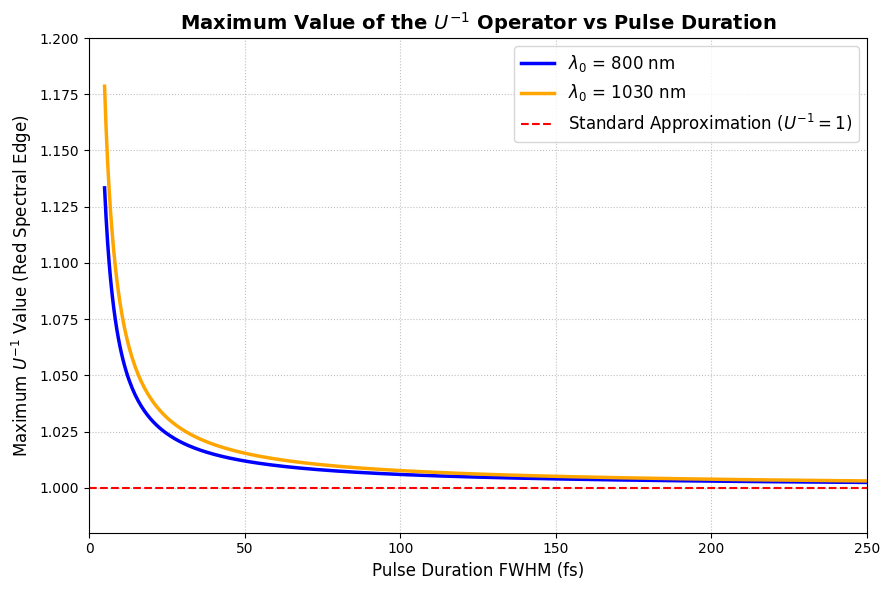
\includegraphics[width=1\linewidth]{dependance U.png}
    \caption{Maximum value of the optical shock operator $\hat{U}^{-1}$ evaluated as a function of the pulse duration (FWHM). The curves compare transform-limited pulses centered at $\lambda_0 = 800$~nm and $1030$~nm. For durations $\tau > 100$~fs, the operator converges to 1, validating the standard approximation $\hat{U}^{-1} \approx 1$. In the few-cycle regime, the deviation becomes significant, particularly for longer central wavelengths.}
    \label{fig:dependance}
\end{figure}

\subsection{Carrier Density Rate Equations}

The code integrates two coupled populations, the free electron density $N$ and the self-trapped exciton density $N_{STE}$, following the two population model of Mao et al.~\cite{mao2004}:
\begin{align}
\frac{dN}{dt} =\;
&\underbrace{W_{PI}(I)\left(1-\frac{N}{N_{at}})\right)}_{\text{direct photoionization, depletes available sites}} \nonumber\\[4pt]
&+\;\underbrace{\Big[W_{STE}(I)+\frac{\sigma_\omega}{U_s} I\, N\Big]\frac{N_{STE}}{N_{at}}}_{\text{re-ionization of trapped excitons}} \nonumber\\[4pt]
&+\;\underbrace{\frac{\sigma_\omega}{U_i}\, I\, N\left(1-\frac{N}{N_{at}})\right)}_{\text{avalanche ionization}}
\;-\;\underbrace{\frac{N}{\tau_r}}_{\text{trapping into the STE channel}}
\end{align}
\begin{align}
\frac{dN_{STE}}{dt} =\;
&\underbrace{\frac{N}{\tau_r}}_{\text{trapping}}
\;-\;\underbrace{\Big[W_{STE}(I)+\frac{\sigma_\omega}{U_s} I\, N\Big]\frac{N_{STE}}{N_{at}}}_{\text{re-ionization}}
\;-\;\underbrace{\frac{N_{STE}}{\tau_{STE}}}_{\text{decay to the ground state}}
\end{align}
Here $I=|\mathcal{E}|^2$ is the local intensity, $W_{STE}$ is the same Keldysh formula evaluated at the smaller gap $U_s$ of the self-trapped state instead of $U_i$, and $\sigma_\omega/U_i =\beta_g$ is the avalanche coefficient with $\beta_s$ its counterpart for the STE channel.

The two populations exchange carriers in both directions. Trapping process moves the electrons out of the conduction band into the STE "band" at the rate $N/\tau_r$, and that same quantity reappears as a gain term in the second equation, so nothing is lost in the transfer. Laser driven re-ionization sends them back the other way, and again the term appears with opposite signs in the two equations. Only the last term of the second equation, $-N_{STE}/\tau_{STE}$, genuinely removes carriers from the pair of populations, since it returns them to the ground state. The kernel also rescales both populations if their sum ever exceeds $N_{at}$, which keeps the model from producing more carriers than there are sites.
\newline

The trapping time $\tau_r$, about $150\ \text{fs}$ in fused silica, is how fast a conduction band electron falls into a self-trapped state.

The relaxation time $\tau_{STE}$, about $1\ \text{ps}$, is how long that trapped state then survives before decaying non radiatively to the ground state. 

\subsection{Bound Polarizability of Self-Trapped Excitons}
Unlike conduction band electrons, self-trapped excitons do not act as free carriers. An STE corresponds to a pair of dangling bonds ($\text{Si}^\bullet$ and $\text{O}^\bullet$) created by the rupture of an $\text{Si}-\text{O}-\text{Si}$ bond. Because their unpaired orbitals lie within the band gap rather than in the conduction band, STEs cannot drift under the influence of the electric field and therefore do not contribute to the Drude free-carrier response. 

Instead, STEs respond to the light field as bound oscillators. Their polarization is governed by a resonance associated with their first excited level, following the formulation of Mao et al.~\cite{mao2004}:
\begin{equation}
\Delta n_{STE} = \frac{N_{STE} \, e^2}{2n_0m_e \varepsilon_0} \, \frac{1}{\omega_{tr}^2 - \omega^2}
\end{equation}
This contribution enters the field equation as the fifth line of Eq.~\eqref{eq:master_propagation}. Since the pump photon energy ($1.55\text{ eV}$) is far below the STE resonance ($\omega_0 < \omega_{tr}$), this term acts purely as a phase contribution with no associated absorption loss. Consequently, it is positive and adds to the Kerr self-focusing rather than opposing it. This mechanism accounts for the permanent, fracture-free refractive index change classified by Couairon et al. as type I damage.

\subsection{Article Reproduction}
In the process of building up the simulation I tried to reproduce several formulas from founding papers.
In the earliest version the program had hard time converging and the calculations were too long to be computed on my computer even with an GPU (graphic process units) optimized calculation. The reason for such problems were firstly that the equations are non linear and such equations have a tendency to showcase chaotic behaviour and are highly sensitive to initial conditions. In the simulation the high intensity beam provokes a sudden peak in free carriers concentration. If the integration cells are too wide, the energy viewed by the cells is diluted, lowering the actual concentration or electricity field intensity. We observe numerical damping. With a finer grid such problems are resolved but the calculation time explodes. Numerical solutions exist but remain hard to implement especially with a cylindrical referential (mesh refinement). It is also important to mention that the intensity levels are so high that the data type themselves becomes the source of error. A calculation using complex numbers coded onto 64 bits were a source of error in the calculation. The mantis associated was not large enough to describe the intensity and caused catastrophic error. Moving to larger data types such as complex 128 worked well, but the issue is that few computers have access to large amounts of these computation units, even super expensive gaming graphics. cards that were in the lab. The only GPU capable of dealing with such data types at a fast speed were so-called professional GPUs, mostly used nowadays to train AI models and that could be found onto data centers.
After several runs of more than twenty hours, it became clear that trial and error techniques were not the most suited for the simulation. After discussing with Prof.Konishi we opted for a cloud computing company, charging 1,51$\$$hour for a Nvidia A100, that allows us to manipulate such calculations in a duration including from 2h down to 6 min depending on the version of the simulation. I would like to thank Prof. Konishi for investing 150$\$$ onto the platform so I can keep researching and improving the simulation.
The current issue with the work is that the simulation poorly deals with out of range intensity (where the material is sublimed) and the simulation keeps working with the out of range step to generate the following which is wrong according to common sense.

Yet at low power it becomes possible to replicate many results from Couairon and Al. article which is a quantitative benchmark needed to push the work further with higher power, different focalisation settings, pump wavelength and introduction of the STE into the model.

Here are some comparative results.


\begin{figure}[htbp]
    \centering
    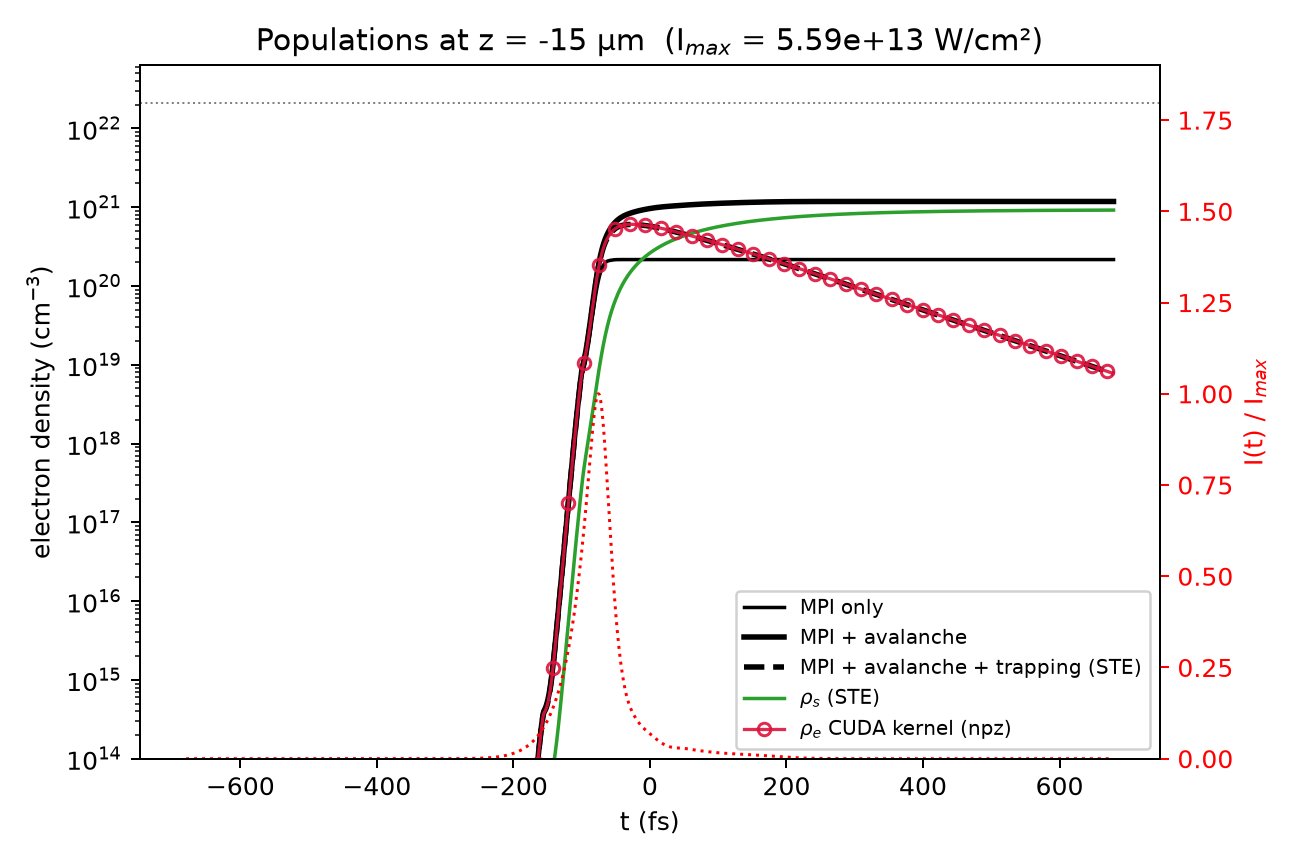
\includegraphics[width=0.85\linewidth]{fig2_populations.png}
    \caption{On-axis electron populations at the nonlinear focus for the $800\ \text{nm}$, $1.1\ \mu$J case, reintegrating the 0D rate equations using the saved temporal intensity profile $I(t)$ under three progressive models (MPI only, then including avalanche, and finally the full model with trapping). Physically, this graph illustrates the critical competition between carrier generation and loss: while multi-photon ionization and avalanche rapidly pump electrons into the conduction band, trapping into self-trapped states ($N_{STE}$, green curve) acts as a powerful brake just after the pulse peak, draining free electrons (dashed black curve) and preventing catastrophic plasma runaway.}
    \label{fig:fig2_populations}
\end{figure}

\begin{figure}[htbp]
    \centering
    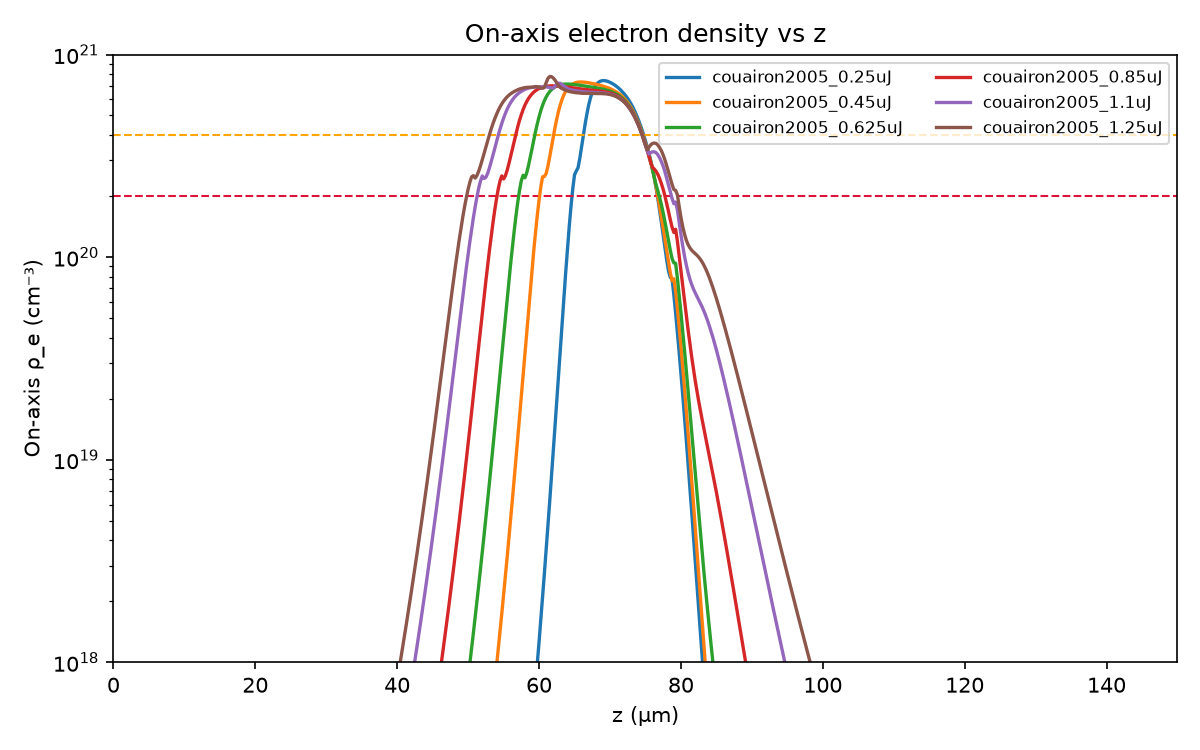
\includegraphics[width=0.85\linewidth]{couairon2005_fig9_energy_sweep.png}
    \caption{On-axis electron density along $z$ for six input energies, reproducing Fig.~9 of~\cite{PhysRevB.71.125435}. Intuitively, this reveals the self-limiting nature of laser filamentation: no matter how much you increase the incoming pulse energy beyond the critical threshold, the peak plasma density refuses to grow indefinitely and saturates around a universal plateau (marked by the dashed reference lines). This clamping effect arises from a direct dynamic feedback loop—as the intensity tries to rise due to Kerr self-focusing, it aggressively triggers ionization, generating a dense plasma cloud ($\sigma_\omega N \mathcal{E}$) that defocuses the beam before it can collapse further.}
    \label{fig:fig9_energy_sweep}
\end{figure}
\begin{figure}[htbp]
    \centering
    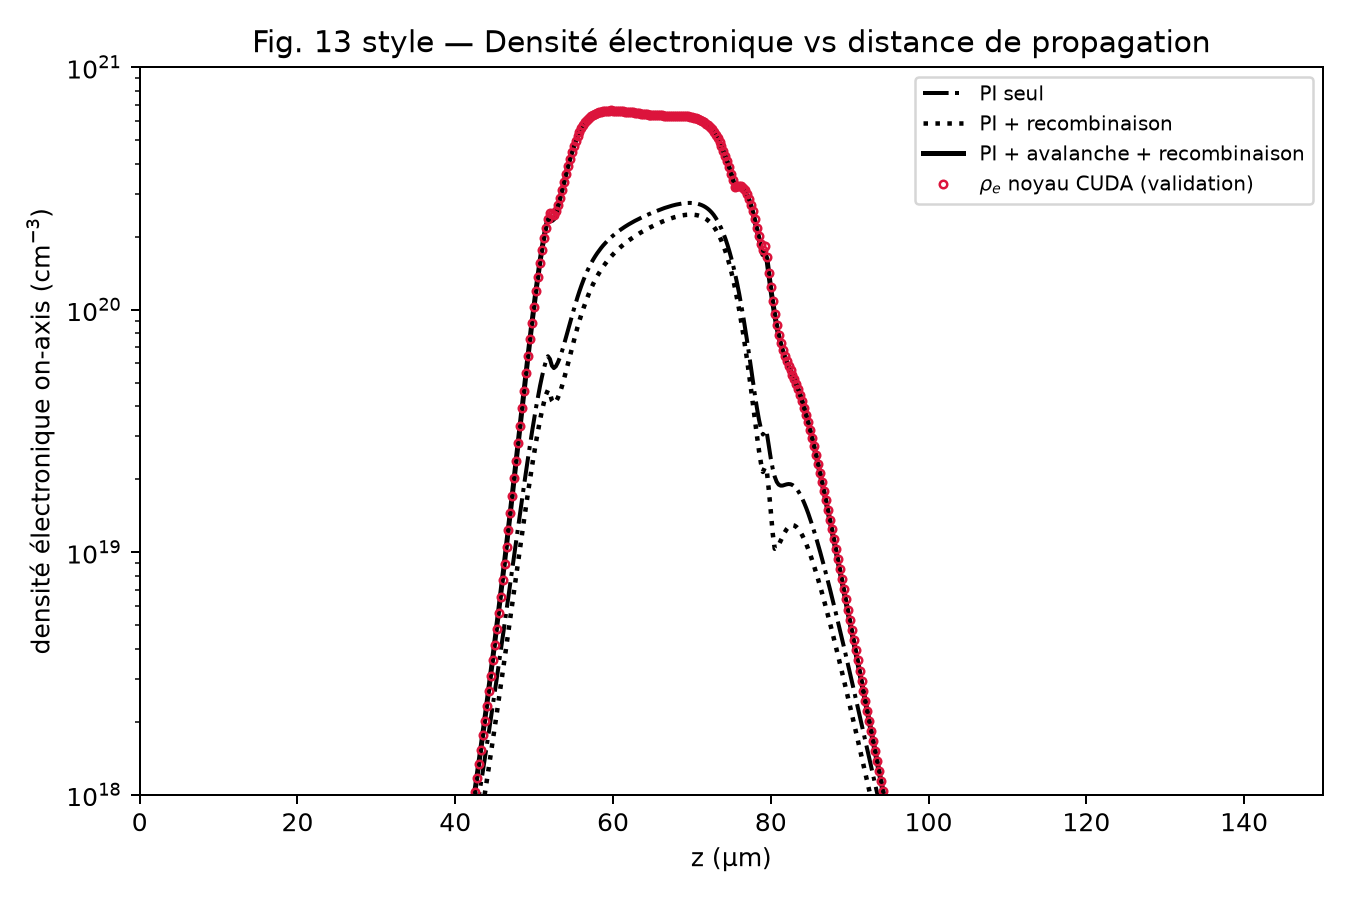
\includegraphics[width=0.85\linewidth]{fig13_electron_density_vs_z.png}
    \caption{On-axis electron density along $z$ at fixed input energy ($1.1\ \mu$J), comparing photoionization only, photoionization with recombination, and the full model including avalanche ionization, against the CUDA kernel output (open circles, reproducing Fig.~13 of~\cite{PhysRevB.71.125435}). Looking at the stark difference between the curves, it becomes clear why MPI alone is fundamentally insufficient: photoionization sets the initial "seed" electrons, but without the avalanche term ($\beta_g I N$) providing exponential multiplication as the intensity climbs, the plasma yield falls orders of magnitude short of reality. Avalanche ionization is therefore the physical engine that turns a weak perturbative absorption into a dense, macroscopic plasma shield.}
    \label{fig:fig13_electron_density}
\end{figure}